% Options for packages loaded elsewhere
\PassOptionsToPackage{unicode}{hyperref}
\PassOptionsToPackage{hyphens}{url}
\PassOptionsToPackage{dvipsnames,svgnames,x11names}{xcolor}
%
\documentclass[
  a4paper,
  DIV=11,
  numbers=noendperiod]{scrartcl}

\usepackage{amsmath,amssymb}
\usepackage{iftex}
\ifPDFTeX
  \usepackage[T1]{fontenc}
  \usepackage[utf8]{inputenc}
  \usepackage{textcomp} % provide euro and other symbols
\else % if luatex or xetex
  \usepackage{unicode-math}
  \defaultfontfeatures{Scale=MatchLowercase}
  \defaultfontfeatures[\rmfamily]{Ligatures=TeX,Scale=1}
\fi
\usepackage{lmodern}
\ifPDFTeX\else  
    % xetex/luatex font selection
\fi
% Use upquote if available, for straight quotes in verbatim environments
\IfFileExists{upquote.sty}{\usepackage{upquote}}{}
\IfFileExists{microtype.sty}{% use microtype if available
  \usepackage[]{microtype}
  \UseMicrotypeSet[protrusion]{basicmath} % disable protrusion for tt fonts
}{}
\makeatletter
\@ifundefined{KOMAClassName}{% if non-KOMA class
  \IfFileExists{parskip.sty}{%
    \usepackage{parskip}
  }{% else
    \setlength{\parindent}{0pt}
    \setlength{\parskip}{6pt plus 2pt minus 1pt}}
}{% if KOMA class
  \KOMAoptions{parskip=half}}
\makeatother
\usepackage{xcolor}
\setlength{\emergencystretch}{3em} % prevent overfull lines
\setcounter{secnumdepth}{-\maxdimen} % remove section numbering
% Make \paragraph and \subparagraph free-standing
\makeatletter
\ifx\paragraph\undefined\else
  \let\oldparagraph\paragraph
  \renewcommand{\paragraph}{
    \@ifstar
      \xxxParagraphStar
      \xxxParagraphNoStar
  }
  \newcommand{\xxxParagraphStar}[1]{\oldparagraph*{#1}\mbox{}}
  \newcommand{\xxxParagraphNoStar}[1]{\oldparagraph{#1}\mbox{}}
\fi
\ifx\subparagraph\undefined\else
  \let\oldsubparagraph\subparagraph
  \renewcommand{\subparagraph}{
    \@ifstar
      \xxxSubParagraphStar
      \xxxSubParagraphNoStar
  }
  \newcommand{\xxxSubParagraphStar}[1]{\oldsubparagraph*{#1}\mbox{}}
  \newcommand{\xxxSubParagraphNoStar}[1]{\oldsubparagraph{#1}\mbox{}}
\fi
\makeatother


\providecommand{\tightlist}{%
  \setlength{\itemsep}{0pt}\setlength{\parskip}{0pt}}\usepackage{longtable,booktabs,array}
\usepackage{calc} % for calculating minipage widths
% Correct order of tables after \paragraph or \subparagraph
\usepackage{etoolbox}
\makeatletter
\patchcmd\longtable{\par}{\if@noskipsec\mbox{}\fi\par}{}{}
\makeatother
% Allow footnotes in longtable head/foot
\IfFileExists{footnotehyper.sty}{\usepackage{footnotehyper}}{\usepackage{footnote}}
\makesavenoteenv{longtable}
\usepackage{graphicx}
\makeatletter
\def\maxwidth{\ifdim\Gin@nat@width>\linewidth\linewidth\else\Gin@nat@width\fi}
\def\maxheight{\ifdim\Gin@nat@height>\textheight\textheight\else\Gin@nat@height\fi}
\makeatother
% Scale images if necessary, so that they will not overflow the page
% margins by default, and it is still possible to overwrite the defaults
% using explicit options in \includegraphics[width, height, ...]{}
\setkeys{Gin}{width=\maxwidth,height=\maxheight,keepaspectratio}
% Set default figure placement to htbp
\makeatletter
\def\fps@figure{htbp}
\makeatother
% definitions for citeproc citations
\NewDocumentCommand\citeproctext{}{}
\NewDocumentCommand\citeproc{mm}{%
  \begingroup\def\citeproctext{#2}\cite{#1}\endgroup}
\makeatletter
 % allow citations to break across lines
 \let\@cite@ofmt\@firstofone
 % avoid brackets around text for \cite:
 \def\@biblabel#1{}
 \def\@cite#1#2{{#1\if@tempswa , #2\fi}}
\makeatother
\newlength{\cslhangindent}
\setlength{\cslhangindent}{1.5em}
\newlength{\csllabelwidth}
\setlength{\csllabelwidth}{3em}
\newenvironment{CSLReferences}[2] % #1 hanging-indent, #2 entry-spacing
 {\begin{list}{}{%
  \setlength{\itemindent}{0pt}
  \setlength{\leftmargin}{0pt}
  \setlength{\parsep}{0pt}
  % turn on hanging indent if param 1 is 1
  \ifodd #1
   \setlength{\leftmargin}{\cslhangindent}
   \setlength{\itemindent}{-1\cslhangindent}
  \fi
  % set entry spacing
  \setlength{\itemsep}{#2\baselineskip}}}
 {\end{list}}
\usepackage{calc}
\newcommand{\CSLBlock}[1]{\hfill\break\parbox[t]{\linewidth}{\strut\ignorespaces#1\strut}}
\newcommand{\CSLLeftMargin}[1]{\parbox[t]{\csllabelwidth}{\strut#1\strut}}
\newcommand{\CSLRightInline}[1]{\parbox[t]{\linewidth - \csllabelwidth}{\strut#1\strut}}
\newcommand{\CSLIndent}[1]{\hspace{\cslhangindent}#1}

\KOMAoption{captions}{tableheading}
\makeatletter
\@ifpackageloaded{tcolorbox}{}{\usepackage[skins,breakable]{tcolorbox}}
\@ifpackageloaded{fontawesome5}{}{\usepackage{fontawesome5}}
\definecolor{quarto-callout-color}{HTML}{909090}
\definecolor{quarto-callout-note-color}{HTML}{0758E5}
\definecolor{quarto-callout-important-color}{HTML}{CC1914}
\definecolor{quarto-callout-warning-color}{HTML}{EB9113}
\definecolor{quarto-callout-tip-color}{HTML}{00A047}
\definecolor{quarto-callout-caution-color}{HTML}{FC5300}
\definecolor{quarto-callout-color-frame}{HTML}{acacac}
\definecolor{quarto-callout-note-color-frame}{HTML}{4582ec}
\definecolor{quarto-callout-important-color-frame}{HTML}{d9534f}
\definecolor{quarto-callout-warning-color-frame}{HTML}{f0ad4e}
\definecolor{quarto-callout-tip-color-frame}{HTML}{02b875}
\definecolor{quarto-callout-caution-color-frame}{HTML}{fd7e14}
\makeatother
\makeatletter
\@ifpackageloaded{caption}{}{\usepackage{caption}}
\AtBeginDocument{%
\ifdefined\contentsname
  \renewcommand*\contentsname{Table of contents}
\else
  \newcommand\contentsname{Table of contents}
\fi
\ifdefined\listfigurename
  \renewcommand*\listfigurename{List of Figures}
\else
  \newcommand\listfigurename{List of Figures}
\fi
\ifdefined\listtablename
  \renewcommand*\listtablename{List of Tables}
\else
  \newcommand\listtablename{List of Tables}
\fi
\ifdefined\figurename
  \renewcommand*\figurename{Figure}
\else
  \newcommand\figurename{Figure}
\fi
\ifdefined\tablename
  \renewcommand*\tablename{Table}
\else
  \newcommand\tablename{Table}
\fi
}
\@ifpackageloaded{float}{}{\usepackage{float}}
\floatstyle{ruled}
\@ifundefined{c@chapter}{\newfloat{codelisting}{h}{lop}}{\newfloat{codelisting}{h}{lop}[chapter]}
\floatname{codelisting}{Listing}
\newcommand*\listoflistings{\listof{codelisting}{List of Listings}}
\makeatother
\makeatletter
\makeatother
\makeatletter
\@ifpackageloaded{caption}{}{\usepackage{caption}}
\@ifpackageloaded{subcaption}{}{\usepackage{subcaption}}
\makeatother

\ifLuaTeX
\usepackage[bidi=basic]{babel}
\else
\usepackage[bidi=default]{babel}
\fi
\babelprovide[main,import]{american}
% get rid of language-specific shorthands (see #6817):
\let\LanguageShortHands\languageshorthands
\def\languageshorthands#1{}
\ifLuaTeX
  \usepackage{selnolig}  % disable illegal ligatures
\fi
\usepackage{bookmark}

\IfFileExists{xurl.sty}{\usepackage{xurl}}{} % add URL line breaks if available
\urlstyle{same} % disable monospaced font for URLs
\hypersetup{
  pdftitle={Analog Circuit Design},
  pdfauthor={Harald Pretl; Michael Koefinger},
  pdflang={en-US},
  colorlinks=true,
  linkcolor={blue},
  filecolor={Maroon},
  citecolor={Blue},
  urlcolor={Blue},
  pdfcreator={LaTeX via pandoc}}


\title{Analog Circuit Design}
\author{Harald Pretl \and Michael Koefinger}
\date{2024-08-02}

\begin{document}
\maketitle

\renewcommand*\contentsname{Table of contents}
{
\hypersetup{linkcolor=}
\setcounter{tocdepth}{3}
\tableofcontents
}

\subsection{Introduction}\label{sec-intro}

This is the material for an intermediate-level MOSFET circuit design
course, held at JKU under course number 336.009 (``KV Analoge
Schaltungstechnik'').

The course makes heavy use of circuit simulation, using \textbf{Xschem}
for schematic entry and \textbf{ngspice} for simulation. The 130nm CMOS
technology \textbf{SG13G2} from IHP Microelectronics is used.

Tools and PDK are integrated in the \textbf{IIC-OSIC-TOOLS} Docker
image, which will be used during the coursework.

\begin{tcolorbox}[enhanced jigsaw, title=\textcolor{quarto-callout-note-color}{\faInfo}\hspace{0.5em}{Note}, left=2mm, titlerule=0mm, colback=white, toptitle=1mm, toprule=.15mm, colframe=quarto-callout-note-color-frame, opacitybacktitle=0.6, rightrule=.15mm, arc=.35mm, breakable, coltitle=black, colbacktitle=quarto-callout-note-color!10!white, opacityback=0, leftrule=.75mm, bottomtitle=1mm, bottomrule=.15mm]

All course material is made publicly available on GitHub and shared
under the Apache-2.0 license.

\end{tcolorbox}

\subsubsection{IHP's SG13G2 130nm CMOS
Technology}\label{ihps-sg13g2-130nm-cmos-technology}

SG13G2 is the name of a 130nm CMOS technology (strictly speaking BiCMOS)
from IHP Microelectronics. It features low-voltage (thin-oxide) core
MOSFET, high-voltage (thick-oxide) I/O MOSFET, various types of linear
resistors, and 7 layers of Aluminium metallization (5 thin plus 2 thick
metal layers). This PDK is open-source, and the complete process
specification can be found at
\href{https://github.com/IHP-GmbH/IHP-Open-PDK/blob/main/ihp-sg13g2/libs.doc/doc/SG13G2_os_process_spec.pdf}{SG13G2
process specification}. While we will not do layouts in this course, the
layout rules can be found at
\href{https://github.com/IHP-GmbH/IHP-Open-PDK/blob/main/ihp-sg13g2/libs.doc/doc/SG13G2_os_layout_rules.pdf}{SG13G2
layout rules}.

For our circuit design, the most important parameters of the available
devices are summarized in the following:

\begin{itemize}
\tightlist
\item
  \textbf{Low-voltage NMOS}: Device \texttt{sg13\_lv\_nmos}; operating
  voltage nominal \(V_\mathrm{DD}=1.5\,\text{V}\),
  \(L_\mathrm{min}=0.13\,\mu\text{m}\),
  \(V_\mathrm{th} \approx 0.5\,\text{V}\); a triple-well option for the
  NMOS is available.
\item
  \textbf{Low-voltage PMOS}: Device \texttt{sg13\_lv\_pmos}; operating
  voltage nominal \(V_\mathrm{DD}=1.5\,\text{V}\),
  \(L_\mathrm{min}=0.13\,\mu\text{m}\),
  \(V_\mathrm{th} \approx -0.47\,\text{V}\).
\item
  \textbf{High-voltage NMOS}: Device \texttt{sg13\_hv\_nmos}; operating
  voltage nominal \(V_\mathrm{DD}=3.3\,\text{V}\),
  \(L_\mathrm{min}=0.45\,\mu\text{m}\),
  \(V_\mathrm{th} \approx 0.7\,\text{V}\); a triple-well option for the
  NMOS is available.
\item
  \textbf{High-voltage PMOS}: Device \texttt{sg13\_hv\_pmos}; operating
  voltage nominal \(V_\mathrm{DD}=3.3\,\text{V}\),
  \(L_\mathrm{min}=0.45\,\mu\text{m}\),
  \(V_\mathrm{th} \approx -0.65\,\text{V}\).
\item
  \textbf{Silicided poly resistor}: Device \texttt{rsil};
  \(R_\square=7\,\Omega \pm 10\%\), \(\mathrm{TC}_1=3100\,\text{ppm/K}\)
\item
  \textbf{Poly resistor}: Device \texttt{rppd};
  \(R_\square=260\,\Omega \pm 10\%\),
  \(\mathrm{TC}_1=170\,\text{ppm/K}\)
\item
  \textbf{Poly resistor high}: Device \texttt{rhigh};
  \(R_\square=1360\,\Omega \pm 15\%\),
  \(\mathrm{TC}_1=-2300\,\text{ppm/K}\)
\item
  \textbf{MIM capacitor}: Device \texttt{cap\_cmim};
  \(C'=1.5\,\text{fF}/\mu\text{m}^2 \pm 10\%\),
  \(\mathrm{VC}_1=-26\text{ppm/V}\), \(\mathrm{TC}_1=3.6\text{ppm/K}\),
  breakdown voltage \(>15\,\mathrm{V}\)
\item
  \textbf{MOM capacitor}: The metal stack is well-suited for MOM
  capacitors due to 5 thin metal layers, but no primitive capacitor
  device is available at this point.
\end{itemize}

\subsubsection{Schematic Entry Using
Xschem}\label{schematic-entry-using-xschem}

Xschem is an open-source schematic entry tool with emphasis on
integrated circuits. For up-to-date information of the many features of
Xschem and the basic operation of it please look at the available
\href{https://xschem.sourceforge.io/stefan/xschem_man/xschem_man.html}{online
documentation}. Usage of Xschem will be learned with the first few basic
examples, essentially using a single MOSFET. The usage model of Xschem
is that the schematic is hierarchically drawn, and the simulation and
evaluation statements are contained in the schematics. Further, Xschem
offers embedded graphing, which we will mostly use.

\subsubsection{Circuit Simulation Using
ngspice}\label{circuit-simulation-using-ngspice}

ngspice is an open-source circuit simulator with SPICE dependency (Nagel
1975). Besides the usual simulated types like \texttt{op} (operating
point), \texttt{dc} (dc sweeps), \texttt{tran} (time-domain), or
\texttt{ac} (small-signal frquency sweeps), ngspice offers a script-like
control interface, where many different simulation controls and result
evaluations can be done. For detailed information please refer to the
latest
\href{https://ngspice.sourceforge.io/docs/ngspice-43-manual.pdf}{online
manual}.

\subsubsection{Integrated IC Design Environment
(IIC-OSIC-TOOLS)}\label{integrated-ic-design-environment-iic-osic-tools}

In order to make use of the various required components (tools like
Xschem and ngspice, PDKs like SG13G2) easier, we will use the
\textbf{IIC-OSIC-TOOLS}. This is a pre-compiled Docker image which
allows to do circuit design on a virtual machine on virtually any type
of computing equipment (personal PC, Raspberry Pi, cloud server) on
various operating systems (Windows, macOS, Linux). For further
information like installed tools, how to setup a VM, etc. please look at
\href{https://github.com/iic-jku/IIC-OSIC-TOOLS}{IIC-OSIC-TOOLS GitHub
page}.

\begin{tcolorbox}[enhanced jigsaw, title=\textcolor{quarto-callout-tip-color}{\faLightbulb}\hspace{0.5em}{Tip}, left=2mm, titlerule=0mm, colback=white, toptitle=1mm, toprule=.15mm, colframe=quarto-callout-tip-color-frame, opacitybacktitle=0.6, rightrule=.15mm, arc=.35mm, breakable, coltitle=black, colbacktitle=quarto-callout-tip-color!10!white, opacityback=0, leftrule=.75mm, bottomtitle=1mm, bottomrule=.15mm]

Please make sure to receive information about your personal VM access
ahead of the course start.

\end{tcolorbox}

Experienced users can install this image on their personal computer, for
JKU students the IIC will host a VM on our compute cluster and provide
personal login credentials.

\begin{tcolorbox}[enhanced jigsaw, title=\textcolor{quarto-callout-note-color}{\faInfo}\hspace{0.5em}{Note}, left=2mm, titlerule=0mm, colback=white, toptitle=1mm, toprule=.15mm, colframe=quarto-callout-note-color-frame, opacitybacktitle=0.6, rightrule=.15mm, arc=.35mm, breakable, coltitle=black, colbacktitle=quarto-callout-note-color!10!white, opacityback=0, leftrule=.75mm, bottomtitle=1mm, bottomrule=.15mm]

In this course, we assume that students have a basic knowledge of Linux
and how to operate it using the terminal. If you are not yet familiar
with Linux (which is basically a must when doing integrated circuit
design as many tools are only available on Linux), then please check out
a Linux introductory course or tutorial online, there are many
ressources available.

\end{tcolorbox}

\subsection{First Steps}\label{first-steps}

In this first chapter we will learn to use Xschem for schematic entry,
and how to operate the ngspice SPICE simulator for circuit simulations.
Further, we will make ourself familiar with the transistor and other
passive components available in the IHP Microelectronics SG13G2
technology. While this is strictly speaking a BiCMOS technology offering
MOSFETs as well as SiGe HBTs, we will use it as a pure CMOS technology.

\subsubsection{The Metal-Oxide-Semiconductor Field-Effect-Transistor
(MOSFET)}\label{sec-mosfet}

In this course, we will not dive into semiconductor physics and derive
the device operation bottom-up starting from a fundamental level
governed by quantum mechanics. Instead, we will treat the MOSFET as a
macroscopic by assuming we have a 4-terminal device, and the performance
of this device regarding its terminal voltages and currents we will
largely derive from the simulation model.

The circuit symbol that we will use for the n-channel MOSFET is shown in
Figure~\ref{fig-nmos-symbol}, and for the p-channel MOSFET it is shown
in Figure~\ref{fig-pmos-symbol}. A control voltage between gate (``G'')
and source (``S'') causes a current to flow between drain (``D'') and
source. The MOSFET is a 4-terminal device, so the bulk (``B'') can also
control the drain-source current flow. Often, the bulk is connected to
source, and then the bulk terminal is not shown to declutter the
schematics.

\begin{tcolorbox}[enhanced jigsaw, title=\textcolor{quarto-callout-note-color}{\faInfo}\hspace{0.5em}{Note}, left=2mm, titlerule=0mm, colback=white, toptitle=1mm, toprule=.15mm, colframe=quarto-callout-note-color-frame, opacitybacktitle=0.6, rightrule=.15mm, arc=.35mm, breakable, coltitle=black, colbacktitle=quarto-callout-note-color!10!white, opacityback=0, leftrule=.75mm, bottomtitle=1mm, bottomrule=.15mm]

Strictly speaking is the drain-source current of a MOSFET controlled by
the voltage between gate and bulk and the voltage between drain and
source. Since bulk is often connected to source anyway, and many circuit
designers historically were already familiar with the operation of the
bipolar junction transistor, it is common to consider the gate-source
voltage (besides the drain-source voltage) as the controlling voltage.

This focus on gate-source implies that the source is special compared to
the drain. In a typical physical MOSFET, however, the drain and source
are constructed exactly the same, and which terminal is drain, and which
terminal is source, is only determined by the applied voltage
potentials, and can change dynamically during operation (think of a
MOSFET operating as a switch\ldots{} which side is the drain, which side
is the source?).

Unfortunately, this focus on a ``special'' source has made its way into
some MOSFET compact models. The model that is used in SG13G2 luckily
uses the PSP model, which is formulated symmetrically with regards to
drain and source, and is thus very well suited for analog and RF circuit
design. For a detailed understanding of the PSP model please refer to
the
\href{https://www.nxp.com/wcm_documents/models/mos-models/model-psp/psp102p4_summary.pdf}{model
documentation}.

\end{tcolorbox}

\begin{figure}[H]

\centering{

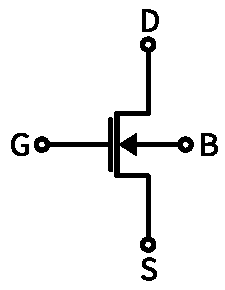
\includegraphics{index_files/mediabag/index_files/figure-pdf/fig-nmos-symbol-output-1.pdf}

}

\caption{\label{fig-nmos-symbol}Circuit symbol of n-channel MOSFET.}

\end{figure}%

\textsubscript{Source:
\href{https://iic-jku.github.io/analog-circuit-design/index.qmd.html}{Article
Notebook}}

\begin{figure}[H]

\centering{

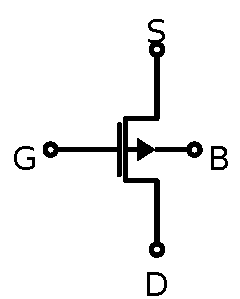
\includegraphics{index_files/mediabag/index_files/figure-pdf/fig-pmos-symbol-output-1.pdf}

}

\caption{\label{fig-pmos-symbol}Circuit symbol of p-channel MOSFET.}

\end{figure}%

\textsubscript{Source:
\href{https://iic-jku.github.io/analog-circuit-design/index.qmd.html}{Article
Notebook}}

For hand calculations and theoretical discussions we will use the
following simplified large-signal model, shown in
Figure~\ref{fig-mosfet-large-signal-model}. A current source
\(I_\mathrm{DS}\) models the current flow between drain and source, and
it is controlled by the three control voltages \(V_\mathrm{GS}\),
\(V_\mathrm{DS}\), and \(V_\mathrm{SB}\). Note that in this way (since
\(I_\mathrm{DS} = f(V_\mathrm{DS})\)) also a resistive behavior between
D and S can be modelled. In case that B and S are shorted then simply
\(V_\mathrm{SB} = 0\).

\textsubscript{Source:
\href{https://iic-jku.github.io/analog-circuit-design/index.qmd.html}{Article
Notebook}}

\begin{figure}[H]

\centering{

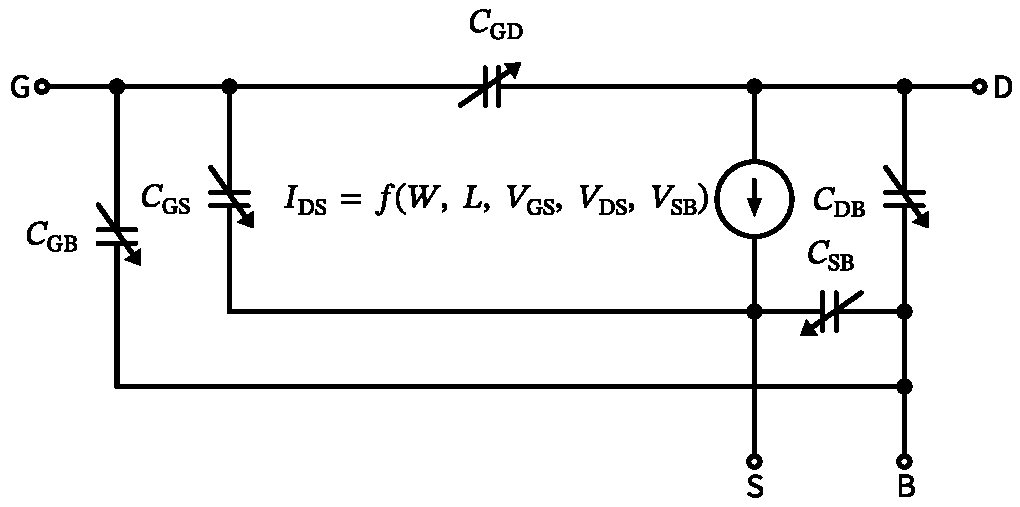
\includegraphics{index_files/mediabag/index_files/figure-pdf/fig-mosfet-large-signal-model-output-1.pdf}

}

\caption{\label{fig-mosfet-large-signal-model}The MOSFET large-signal
model.}

\end{figure}%

\textsubscript{Source:
\href{https://iic-jku.github.io/analog-circuit-design/index.qmd.html}{Article
Notebook}}

In an ideal MOSFET no dc current is flowing into the gate, the behavior
is purely capacitive. We model this by two capacitors:
\(C_\mathrm{GG} = C_\mathrm{GS} + C_\mathrm{GD}\) is the total
capacitance when looking into the gate of the MOSFET. \(C_\mathrm{GS}\)
is usually the dominant capacitance, and \(C_\mathrm{GD}\) models the
capacitive feedback between D and G, usually induced by a topological
overlap capacitance in the physical construction of the MOSFET. This
capacitance is often small compared to \(C_\mathrm{GS}\), but in
situations where we have a large voltage swing at the drain this
capacitance will be affected by the
\href{https://en.wikipedia.org/wiki/Miller_effect}{Miller effect}. In
hand calculations we will often set \(C_\mathrm{GD} = 0\).

\begin{tcolorbox}[enhanced jigsaw, title=\textcolor{quarto-callout-note-color}{\faInfo}\hspace{0.5em}{Note}, left=2mm, titlerule=0mm, colback=white, toptitle=1mm, toprule=.15mm, colframe=quarto-callout-note-color-frame, opacitybacktitle=0.6, rightrule=.15mm, arc=.35mm, breakable, coltitle=black, colbacktitle=quarto-callout-note-color!10!white, opacityback=0, leftrule=.75mm, bottomtitle=1mm, bottomrule=.15mm]

The bulk connection in Figure~\ref{fig-mosfet-large-signal-model} seems
floating as we only consider it a control terminal, where the potential
difference between source and bulk influences the behaviour of the
MOSFET. However, we do not consider resistive or capacitive effects
associated with this node, which is of course a gross simplification,
but nevertheless one we will make in this course.

\end{tcolorbox}

Now, as we are skipping the bottom-up approach of deriving the MOSFET
large-signal behaviour from basic principles, we need to understand the
behaviour of the elements of the large-signal model in
Figure~\ref{fig-mosfet-large-signal-model} by using a circuit simulator
and observing what happens. And generally, a first step in any new IC
technology should be to investigate basic MOSFET performance, by doing
simple dc sweeps of \(V_\mathrm{GS}\) and \(V_\mathrm{DS}\) and looking
at \(I_\mathrm{DS}\) and other large- and small-signal parameters.

As a side note, the students who want to understand MOSFET behaviour
from a physical angle should consult the MOSFET chapter from the JKU
course ``Design of Complex Integrated Circuits'' (VL 336.048). A great
introduction into MOSFET operation and fabrication is given in (Hu
2010), which is available freely
\href{https://www.chu.berkeley.edu/modern-semiconductor-devices-for-integrated-circuits-chenming-calvin-hu-2010/}{online}
and is a recommended read. A very detailed description of the MOSFET
(leaving usually no question unanswered) is provided in (Tsividis and
McAndrew 2011).

Now, in order to get started, basic Xschem testbenches are prepared, and
first simple dc sweeps of various voltages and currents will be done.
But before that, please look at the import note below!

\begin{tcolorbox}[enhanced jigsaw, title=\textcolor{quarto-callout-important-color}{\faExclamation}\hspace{0.5em}{Important}, left=2mm, titlerule=0mm, colback=white, toptitle=1mm, toprule=.15mm, colframe=quarto-callout-important-color-frame, opacitybacktitle=0.6, rightrule=.15mm, arc=.35mm, breakable, coltitle=black, colbacktitle=quarto-callout-important-color!10!white, opacityback=0, leftrule=.75mm, bottomtitle=1mm, bottomrule=.15mm]

Throughout this material, we will stick to the following notations:

\begin{itemize}
\tightlist
\item
  A \textbf{dc quantity} is shown with an upper-case letter with
  upper-case subscripts, like \(V_\mathrm{GS}\).
\item
  Double-subscripts denote \textbf{dc sources}, like \(V_\mathrm{DD}\)
  and \(V_\mathrm{SS}\).
\item
  An \textbf{ac (small-signal) quantity} is a lower-case letter with a
  lower-case subscript, like \(g_\mathrm{m}\).
\item
  A \textbf{total quantity} (dc plus ac) is shown as a lowercase letter
  with upper-case subscript, like \(i_\mathrm{DS}\).
\item
  A upper-case letter with a lower-case subscript is used to denote
  \textbf{RMS quantities}, like \(I_\mathrm{ds}\).
\end{itemize}

\end{tcolorbox}

\paragraph{Large-Signal MOSFET Model}\label{large-signal-mosfet-model}

We start with an investigation into the large-signal MOSFET model shown
in Figure~\ref{fig-mosfet-large-signal-model} by using the simple
testbench for the LV NMOS shown in Figure~\ref{fig-simple-nmos-tb}.

\begin{figure}

\centering{

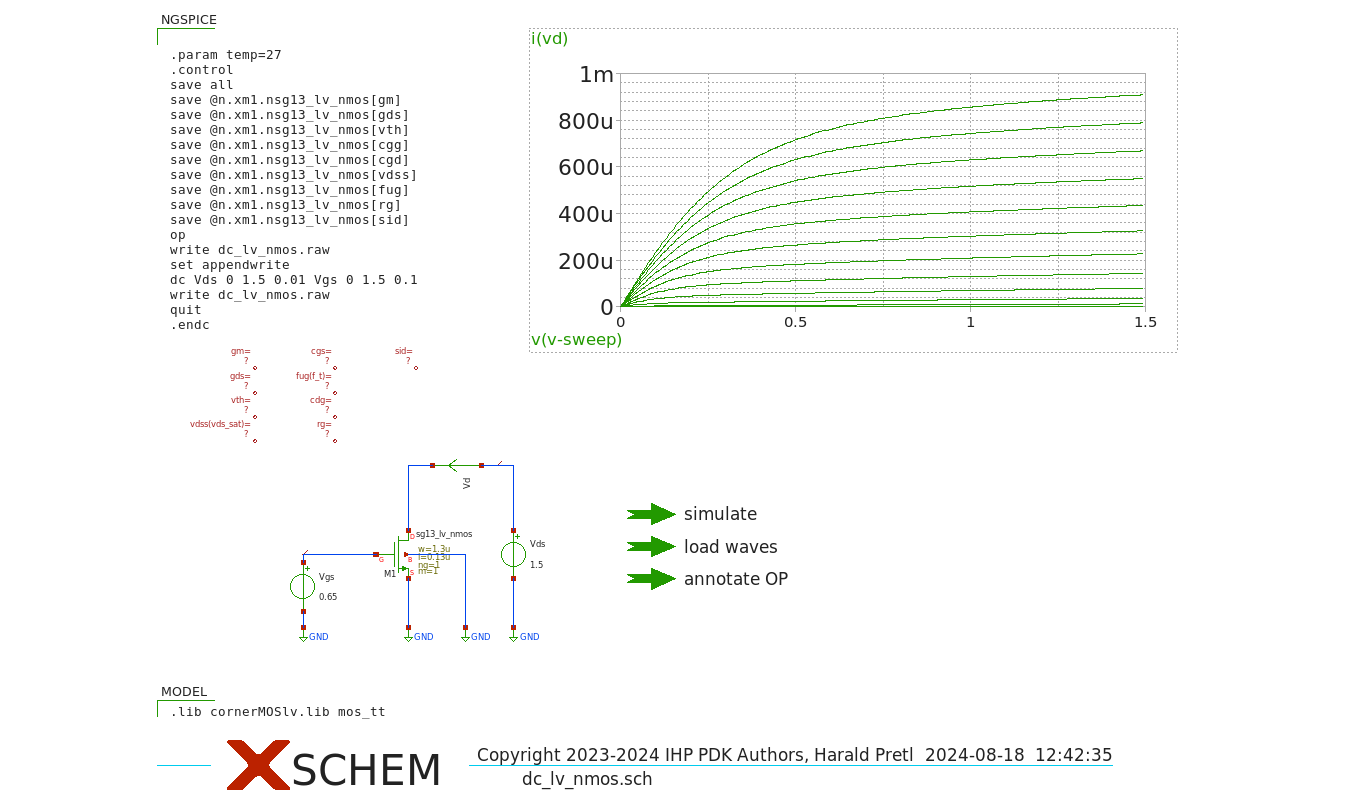
\includegraphics{./xschem/dc_lv_nmos.png}

}

\caption{\label{fig-simple-nmos-tb}Testbench for NMOS dc sweeps.}

\end{figure}%

\begin{tcolorbox}[enhanced jigsaw, title=\textcolor{quarto-callout-tip-color}{\faLightbulb}\hspace{0.5em}{Exercise}, left=2mm, titlerule=0mm, colback=white, toptitle=1mm, toprule=.15mm, colframe=quarto-callout-tip-color-frame, opacitybacktitle=0.6, rightrule=.15mm, arc=.35mm, breakable, coltitle=black, colbacktitle=quarto-callout-tip-color!10!white, opacityback=0, leftrule=.75mm, bottomtitle=1mm, bottomrule=.15mm]

Please try to execute the following steps and answer these questions:

\begin{enumerate}
\def\labelenumi{\arabic{enumi}.}
\tightlist
\item
  Get the LV NMOS testbench (available at
  \url{https://github.com/iic-jku/analog-circuit-design/blob/main/xschem/dc_lv_nmos.sch})
  working in your IIC-OSIC-TOOLS environment.
\item
  Make yourself familiar with Xschem (change the schematic in various
  ways, run a simulation, graph the result).
\item
  Make youself familiar with ngspice (run various simulations, save nets
  and parameters, use the embedded Xschem graphing, explore the
  interactive ngspice shell to look at MOSFET model parameters).
\item
  Explore the LV NMOS \texttt{sg13\_lv\_nmos}:

  \begin{enumerate}
  \def\labelenumii{\arabic{enumii}.}
  \tightlist
  \item
    How is \(I_\mathrm{DS}\) affected by \(V_\mathrm{GS}\) and
    \(V_\mathrm{DS}\)?
  \item
    Change \(W\) and \(L\) of the MOSFET. What is the impact on the
    above parameters? Can you explain the variations?
  \item
    When looking at the model parameters in ngspice, you see that there
    is a \(C_\mathrm{GD}\) and a \(C_\mathrm{DG}\). Why is this, what
    could be the difference? Sometimes these capacitors show a negative
    value, why?
  \end{enumerate}
\item
  Build testbenches in Xschem for the LV PMOS, the HV NMOS, and the HV
  PMOS. Explore the different results.

  \begin{enumerate}
  \def\labelenumii{\arabic{enumii}.}
  \tightlist
  \item
    For a given \(W\) and \(L\), which device provides more drain
    current? How are the capacitances related?
  \item
    If you would have to size an inverter, what would be the ideal ratio
    of \(W_p/W_n\)? Will you exactly design this ratio, or are the
    reasons to deviate?
  \item
    There are LV and HV MOSFETs, and you investigated the difference in
    performance. What is the rationale when designing circuits for
    selection either an LV type, and when to choose an HV type?
  \end{enumerate}
\item
  Build a test bench to explore the body effect, start with LV NMOS.

  \begin{enumerate}
  \def\labelenumii{\arabic{enumii}.}
  \tightlist
  \item
    What happens when \(V_\mathrm{BS} \neq 0\)?
  \end{enumerate}
\end{enumerate}

\end{tcolorbox}

\paragraph{Small-Signal MOSFET Model}\label{small-signal-mosfet-model}

As you have seen in the previous investigations, the large-signal model
of Figure~\ref{fig-mosfet-large-signal-model} describes the behaviour of
the MOSFET across a wide range of voltages applied at the MOSFET
terminals. Unfortunately, for hand analysis dealing with a nonlinear
model is close to impossible, at the very least it is quite tedious.

However, for many practical situations, we bias a MOSFET with a set of
dc voltages applied to its terminal, and only apply small signal
excursions during operation. If we do this, we can linearize the
large-signal model in this dc operating point, and resort to a
small-signal model which can be very useful for hand calculations. Many
experienced designers analyze their circuits by doing these kind of hand
calculations and describing the circuit analytically, which is a great
way to understand fundamental performance limits and relationships
between parameters.

We will use the small-signal MOSFET model shown in
Figure~\ref{fig-mosfet-small-signal-model} for this course. The
current-source \(i_\mathrm{ds} = g_\mathrm{m} v_\mathrm{gs}\) models the
drain current as a function of \(v_\mathrm{gs}\), and the resistor
\(g_\mathrm{ds}\) models the dependency of the drain current by
\(v_\mathrm{ds}\). The drain current dependency on the source-bulk
voltage (the so-called ``body effect'') is introduced by the current
source \(i_\mathrm{ds} = g_\mathrm{mb} v_\mathrm{sb}\).

\textsubscript{Source:
\href{https://iic-jku.github.io/analog-circuit-design/index.qmd.html}{Article
Notebook}}

\begin{figure}[H]

\centering{

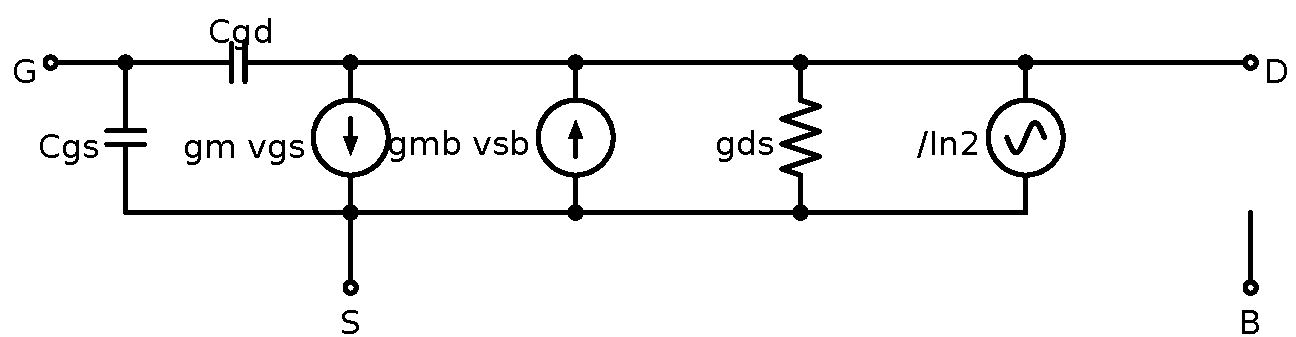
\includegraphics{index_files/mediabag/index_files/figure-pdf/fig-mosfet-small-signal-model-output-1.pdf}

}

\caption{\label{fig-mosfet-small-signal-model}The MOSFET small-signal
model.}

\end{figure}%

\textsubscript{Source:
\href{https://iic-jku.github.io/analog-circuit-design/index.qmd.html}{Article
Notebook}}

As any electronic device the MOSFET introduces noise into the circuit.
In this course we will only consider the drain-source current noise of
the MOSFET, given by
\(\overline{I_\mathrm{n}^2} = 4 k T \gamma g_\mathrm{d0}\)
(\(\overline{I_\mathrm{n}^2}\) is the power-spectral density of the
noise in A\(^2\)/Hz; \(k\) is the Boltzmann constant; \(T\) is the
absolute temperature; \(\gamma\) is a parameter in simplified theory
changing between \(\gamma = 2/3\) in saturation and \(\gamma =1\) for
triode operation; \(g_\mathrm{d0}\) is equal to \(g_\mathrm{m}\) in
saturation and \(g_\mathrm{ds}\) in triode).

\begin{tcolorbox}[enhanced jigsaw, title=\textcolor{quarto-callout-note-color}{\faInfo}\hspace{0.5em}{Note}, left=2mm, titlerule=0mm, colback=white, toptitle=1mm, toprule=.15mm, colframe=quarto-callout-note-color-frame, opacitybacktitle=0.6, rightrule=.15mm, arc=.35mm, breakable, coltitle=black, colbacktitle=quarto-callout-note-color!10!white, opacityback=0, leftrule=.75mm, bottomtitle=1mm, bottomrule=.15mm]

Sometimes we will refer to different operating modes of the MOSFET like
``saturation'' or ``triode''. Generally speaking, when the drain-source
voltage is small, then the MOSFET acts as a resistor, and this mode of
operation we call ``triode'' mode. When the drain-source voltage is
increased, at some point the drain-source current saturates and is no
longer a strong function of the drain-source voltage. This mode is
called ``saturation'' mode. As you can see in the large-signal
investigations, these transitions happen gradually, and it is difficult
to define a precise point where one operating mode switches to the other
one. In this sense we use terms like ``triode'' and ``saturation'' only
in an approximative sense.

\end{tcolorbox}

Now we need to see how the small-signal parameters seen in
Figure~\ref{fig-mosfet-small-signal-model} can be investigated and
estimated using circuit simulation.

\begin{tcolorbox}[enhanced jigsaw, title=\textcolor{quarto-callout-tip-color}{\faLightbulb}\hspace{0.5em}{Exercise}, left=2mm, titlerule=0mm, colback=white, toptitle=1mm, toprule=.15mm, colframe=quarto-callout-tip-color-frame, opacitybacktitle=0.6, rightrule=.15mm, arc=.35mm, breakable, coltitle=black, colbacktitle=quarto-callout-tip-color!10!white, opacityback=0, leftrule=.75mm, bottomtitle=1mm, bottomrule=.15mm]

Please try to execute the following steps and answer the following
questions:

\begin{enumerate}
\def\labelenumi{\arabic{enumi}.}
\tightlist
\item
  Reuse the LV NMOS testbench (available at
  \url{https://github.com/iic-jku/analog-circuit-design/blob/main/xschem/dc_lv_nmos.sch}).
\item
  Explore the LV NMOS \texttt{sg13\_lv\_nmos}:

  \begin{enumerate}
  \def\labelenumii{\arabic{enumii}.}
  \tightlist
  \item
    How are \(g_\mathrm{m}\) and \(g_\mathrm{ds}\) changing when you
    change the dc node voltages?
  \item
    What is the ratio of \(g_\mathrm{m}\) to \(g_\mathrm{mb}\)? What is
    the physical reason behind this ratio (you might want to revisit
    MOSFET device physics at this point)?
  \item
    Take a look at the device capacitances \(C_\mathrm{gs}\) and
    \(C_\mathrm{gd}\). Why are they important? What is the relation to
    \(f_\mathrm{T}\)? \emph{Note: \(f_\mathrm{T}\) is the transit
    frequency where the current gain of the MOSFET drops to 1, and can
    be approximated by
    \(2 \pi f_\mathrm{T} = g_\mathrm{m} / C_\mathrm{gg}\).}
  \item
    Look at the drain noise current according to the MOSFET model and
    compare with a hand calculation of the noise. In the noise equation
    there is the factor \(\gamma\), which in triode is \(\gamma=1\) and
    in saturation is \(\gamma=2/3\) according to basic text books. Which
    value of \(\gamma\) are you calculating? Why might it be different?
  \end{enumerate}
\item
  Go back to your testbench for the LVS PMOS \texttt{sg13\_lv\_pmos}:

  \begin{enumerate}
  \def\labelenumii{\arabic{enumii}.}
  \tightlist
  \item
    What is the difference in \(g_\mathrm{m}\), \(g_\mathrm{ds}\), and
    other parameters between the NMOS and the PMOS? Why could they be
    different?
  \end{enumerate}
\end{enumerate}

\end{tcolorbox}

\paragraph{Conclusion}\label{conclusion}

Congratulations for making it thus far! By now you should have a solid
grasp of the tool handling of Xschem and ngspice, and you should be
familiar with the large- and small-signal operation of both NMOS and
PMOS, and the parameters describing these behaviours. If you feel you
are not sufficiently fluent in these things, please go back to the
beginning of Section~\ref{sec-mosfet} and revisit the relevant sections,
or dive into further reading about the MOSFET operation, like in (Hu
2010).

\subsubsection{First Circuit: MOSFET Diode}\label{sec-mosfet-diode}

This sections need to be written, but here is a first figure.

\textsubscript{Source:
\href{https://iic-jku.github.io/analog-circuit-design/index.qmd.html}{Article
Notebook}}

\begin{figure}[H]

\centering{

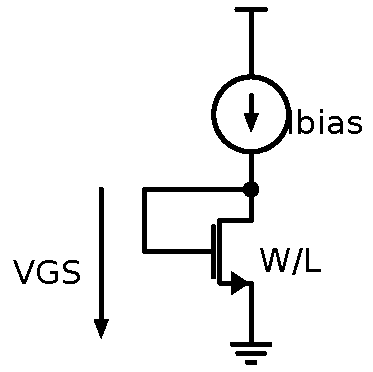
\includegraphics{index_files/mediabag/index_files/figure-pdf/fig-mosfet-diode-output-1.pdf}

}

\caption{\label{fig-mosfet-diode}A MOSFET connected as a diode.}

\end{figure}%

\textsubscript{Source:
\href{https://iic-jku.github.io/analog-circuit-design/index.qmd.html}{Article
Notebook}}

\subsection{Transistor Sizing Using gm/ID
Methodoloy}\label{transistor-sizing-using-gmid-methodoloy}

When designing circuits it is an important question how to select
various parameters of a MOSFET, like \(W\), \(L\), or the bias current
\(I_\mathrm{D}\). As a very practical approach we select the
\(g_\mathrm{m}/I_\mathrm{D}\) methodoloy introduced by P. Jespers and B.
Murmann in (Jespers and Murmann 2017). A brief introduction is available
\href{https://github.com/iic-jku/analog-circuit-design/blob/main/sizing/Ref_Murmann_gmID.pdf}{here}
as well.

\subsubsection{NMOS}\label{nmos}

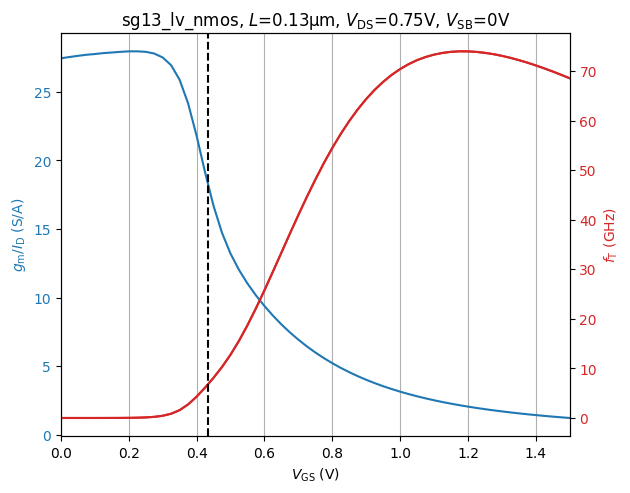
\includegraphics{index_files/figure-latex/.-sizing-techsweep_sg13_plots_nmos-cell-6-output-1.png}

\textsubscript{Source:
\href{https://iic-jku.github.io/analog-circuit-design/index.qmd.html}{Article
Notebook}}

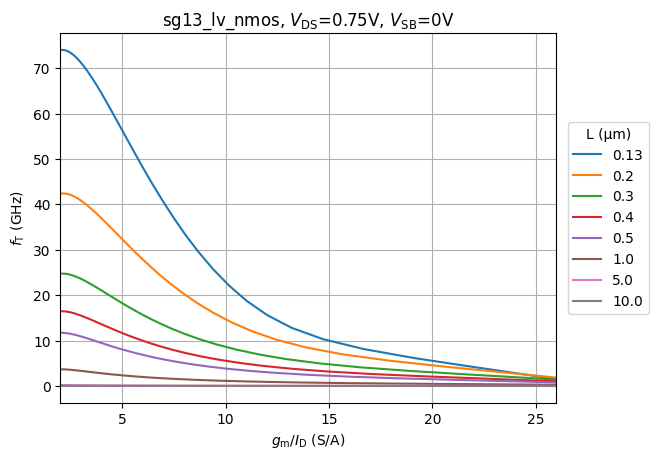
\includegraphics{index_files/figure-latex/.-sizing-techsweep_sg13_plots_nmos-cell-9-output-1.png}

\textsubscript{Source:
\href{https://iic-jku.github.io/analog-circuit-design/index.qmd.html}{Article
Notebook}}

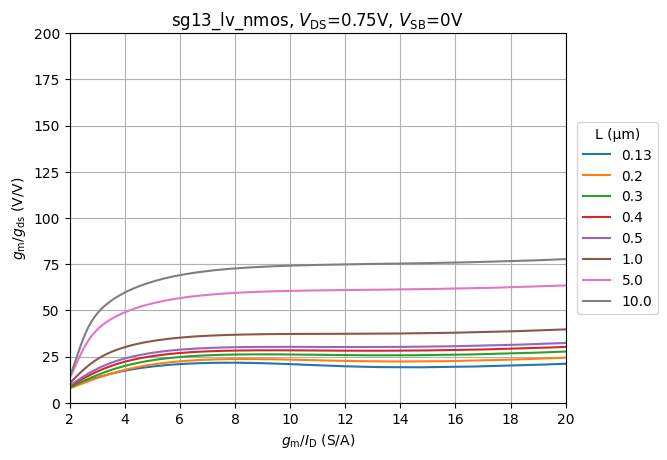
\includegraphics{index_files/figure-latex/.-sizing-techsweep_sg13_plots_nmos-cell-10-output-1.png}

\textsubscript{Source:
\href{https://iic-jku.github.io/analog-circuit-design/index.qmd.html}{Article
Notebook}}

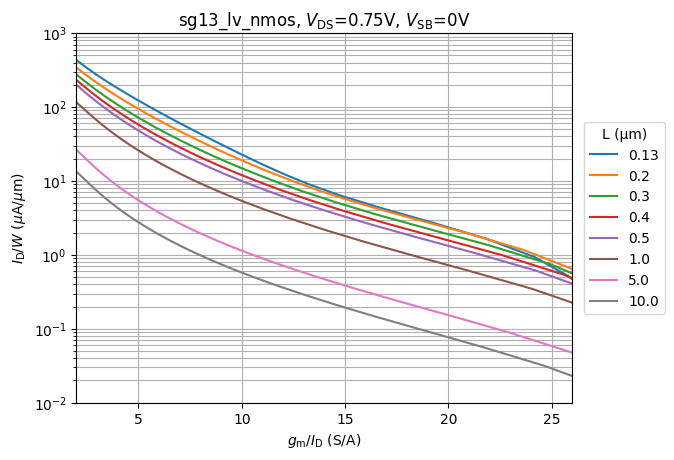
\includegraphics{index_files/figure-latex/.-sizing-techsweep_sg13_plots_nmos-cell-11-output-1.png}

\textsubscript{Source:
\href{https://iic-jku.github.io/analog-circuit-design/index.qmd.html}{Article
Notebook}}

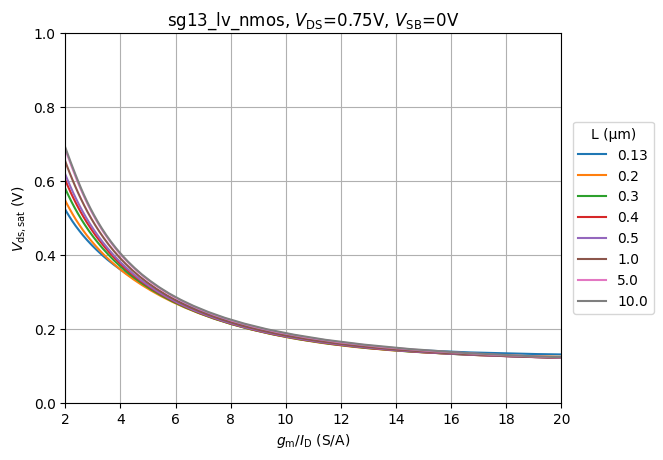
\includegraphics{index_files/figure-latex/.-sizing-techsweep_sg13_plots_nmos-cell-12-output-1.png}

\textsubscript{Source:
\href{https://iic-jku.github.io/analog-circuit-design/index.qmd.html}{Article
Notebook}}

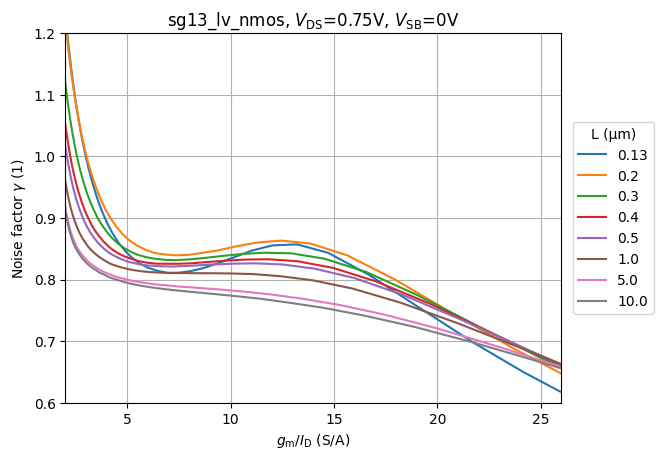
\includegraphics{index_files/figure-latex/.-sizing-techsweep_sg13_plots_nmos-cell-13-output-1.png}

\textsubscript{Source:
\href{https://iic-jku.github.io/analog-circuit-design/index.qmd.html}{Article
Notebook}}

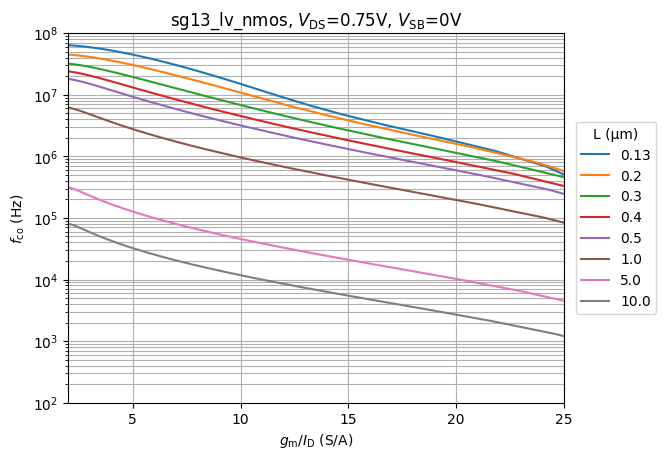
\includegraphics{index_files/figure-latex/.-sizing-techsweep_sg13_plots_nmos-cell-14-output-1.png}

\textsubscript{Source:
\href{https://iic-jku.github.io/analog-circuit-design/index.qmd.html}{Article
Notebook}}

\subsubsection{PMOS}\label{pmos}

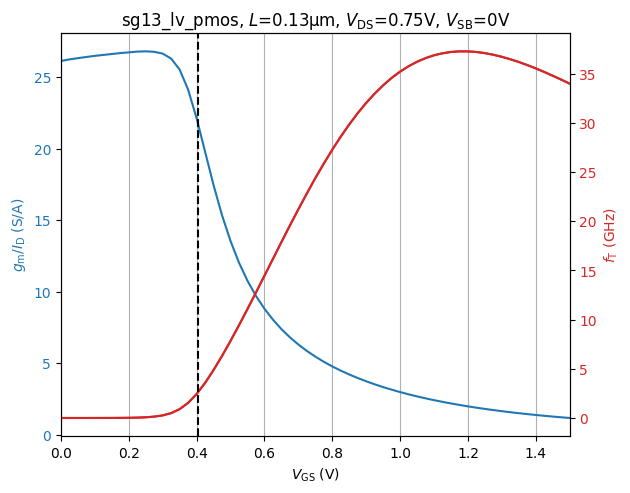
\includegraphics{index_files/figure-latex/.-sizing-techsweep_sg13_plots_pmos-cell-6-output-1.png}

\textsubscript{Source:
\href{https://iic-jku.github.io/analog-circuit-design/index.qmd.html}{Article
Notebook}}

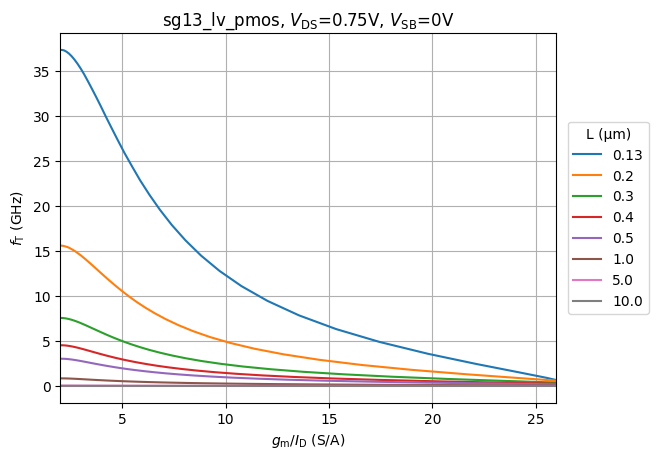
\includegraphics{index_files/figure-latex/.-sizing-techsweep_sg13_plots_pmos-cell-9-output-1.png}

\textsubscript{Source:
\href{https://iic-jku.github.io/analog-circuit-design/index.qmd.html}{Article
Notebook}}

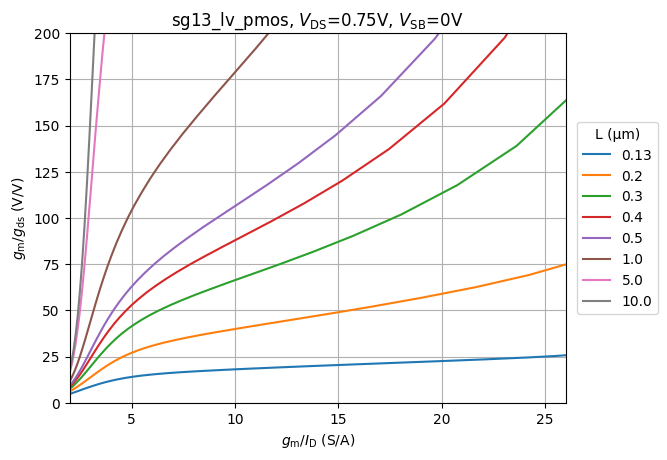
\includegraphics{index_files/figure-latex/.-sizing-techsweep_sg13_plots_pmos-cell-10-output-1.png}

\textsubscript{Source:
\href{https://iic-jku.github.io/analog-circuit-design/index.qmd.html}{Article
Notebook}}

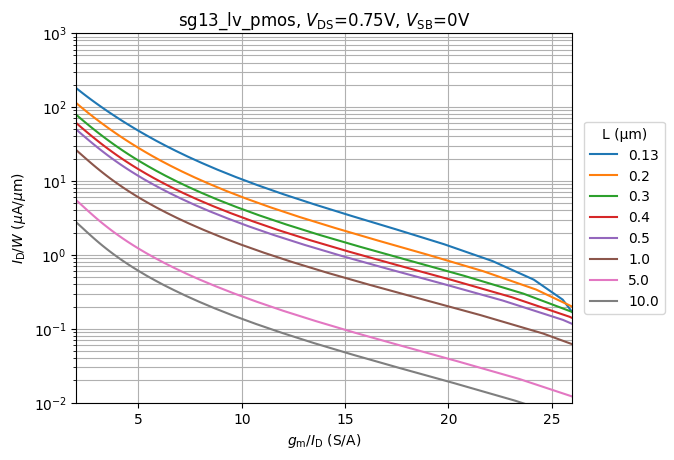
\includegraphics{index_files/figure-latex/.-sizing-techsweep_sg13_plots_pmos-cell-11-output-1.png}

\textsubscript{Source:
\href{https://iic-jku.github.io/analog-circuit-design/index.qmd.html}{Article
Notebook}}

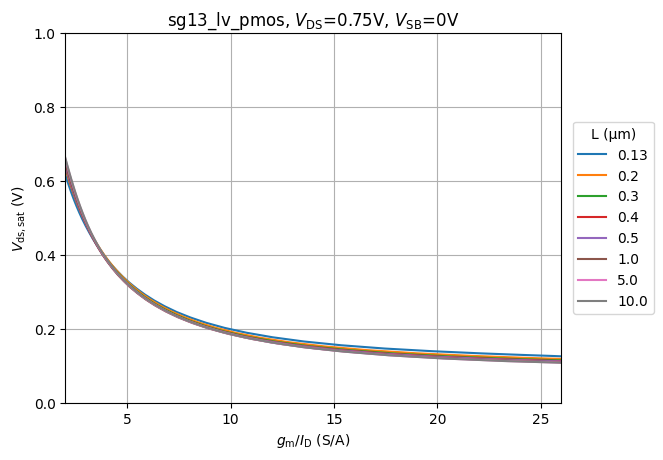
\includegraphics{index_files/figure-latex/.-sizing-techsweep_sg13_plots_pmos-cell-12-output-1.png}

\textsubscript{Source:
\href{https://iic-jku.github.io/analog-circuit-design/index.qmd.html}{Article
Notebook}}

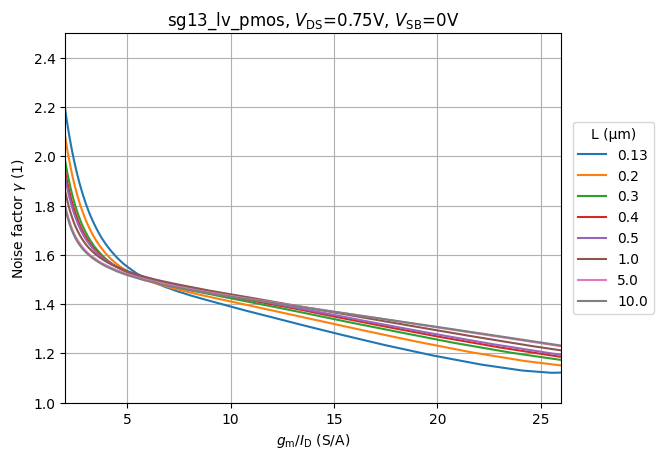
\includegraphics{index_files/figure-latex/.-sizing-techsweep_sg13_plots_pmos-cell-13-output-1.png}

\textsubscript{Source:
\href{https://iic-jku.github.io/analog-circuit-design/index.qmd.html}{Article
Notebook}}

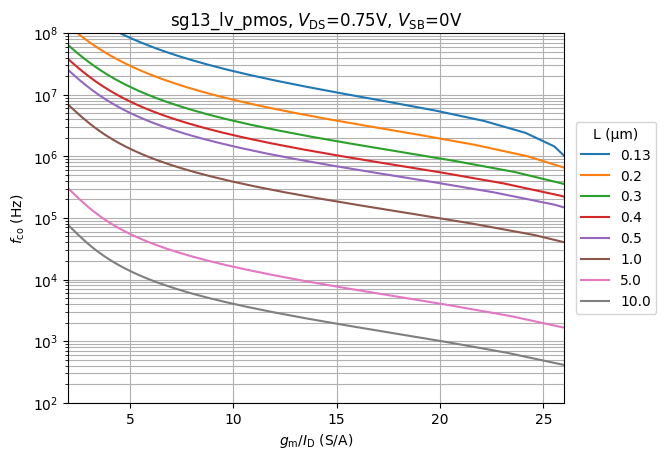
\includegraphics{index_files/figure-latex/.-sizing-techsweep_sg13_plots_pmos-cell-14-output-1.png}

\textsubscript{Source:
\href{https://iic-jku.github.io/analog-circuit-design/index.qmd.html}{Article
Notebook}}

\subsection{Current Mirror}\label{current-mirror}

\subsection{Differential Pair}\label{differential-pair}

\subsection{Cascode Stage}\label{cascode-stage}

\subsection{A Basic 5-Transistor OTA}\label{a-basic-5-transistor-ota}

\subsection{A Fully-Differential OTA}\label{a-fully-differential-ota}

\subsection{Biasing the OTA}\label{biasing-the-ota}

\subsection{An RC-OPAMP Filter}\label{an-rc-opamp-filter}

\subsection{Summary \& Conclusion}\label{summary-conclusion}

\subsection{Appendix: ngspice Cheat
Sheet}\label{appendix-ngspice-cheat-sheet}

\subsection{Appendix: Xschem Cheat
Sheet}\label{appendix-xschem-cheat-sheet}

\textsubscript{Source:
\href{https://iic-jku.github.io/analog-circuit-design/index.qmd.html}{Article
Notebook}}

\phantomsection\label{refs}
\begin{CSLReferences}{1}{0}
\bibitem[\citeproctext]{ref-Chenming_Hu_2010}
Hu, Chenming. 2010. \emph{Modern Semiconductor Devices for Integrated
Circuits}. Pearson.

\bibitem[\citeproctext]{ref-Jespers_Murmann_2017}
Jespers, Paul G. A., and Boris Murmann. 2017. \emph{Systematic Design of
Analog CMOS Circuits: Using Pre-Computed Lookup Tables}. Cambridge
University Press.

\bibitem[\citeproctext]{ref-Nagel_1975}
Nagel, Laurence W. 1975. {``SPICE2: A Computer Program to Simulate
Semiconductor Circuits.''} PhD thesis, EECS Department, University of
California, Berkeley.
\url{http://www2.eecs.berkeley.edu/Pubs/TechRpts/1975/9602.html}.

\bibitem[\citeproctext]{ref-Tsividis_McAndrew_2011}
Tsividis, Yannis, and Colin McAndrew. 2011. \emph{Operation and Modeling
of the MOS Transistor}. Oxford University Press.

\end{CSLReferences}




\end{document}
